\documentclass[aspectratio=169]{beamer}

\usepackage[utf8]{inputenc}
%\usepackage{emoji}

\usepackage{amsmath}
\usepackage{graphicx}
\usepackage[T1]{fontenc}
\usepackage{Oswald}
\usepackage{array}

\usepackage{enumitem}
\setitemize{label=\usebeamerfont*{itemize item}%
  \usebeamercolor[fg]{itemize item}
  \usebeamertemplate{itemize item},
}
\setbeamertemplate{itemize item}[square]
\setbeamertemplate{itemize subitem}[circle]

\usepackage{pgfplots}
\pgfplotsset{compat=1.18}
\usepackage{tikz}
\usepgfplotslibrary{fillbetween}
\usetikzlibrary{patterns}

% \tikzset{
% 	invisible/.style={opacity=0},
% 	visible on/.style={alt={#1{}{invisible}}},
% 	alt/.code args={<#1>#2#3}{%
% 		\alt<#1>{\pgfkeysalso{#2}}{\pgfkeysalso{#3}} % \pgfkeysalso doesn't change the path
% 	},
% }

%\pgfplotsset{every axis/.append style={label style={font=\small},tick label style={font=\footnotesize} }}

\newcommand{\graphheight}{7cm}
\newcommand{\graphwidth}{11cm}

\newcommand{\E}[1]{E\left[#1 \right]}
\newcommand{\ind}[1]{\mathbf{1}_{#1}}

%\newcommand{\P}[1]{E\left[#1\right]}

% \definecolor{azulcito}{RGB}{20,70,140}
\definecolor{azulcito}{RGB}{0,80,150}
\definecolor{verdecito}{RGB}{80,150,0}
\definecolor{rojito}{RGB}{150,0,80}
\definecolor{violetita}{RGB}{150,20,150}


\setbeamercolor*{structure}{fg=azulcito,bg=azulcito!20!white}
\setbeamercolor*{alerted text}{fg=azulcito}

  \setbeamercolor{block title}{fg=azulcito,bg=azulcito!20!white}
  \setbeamercolor{block body}{fg=black,bg=azulcito!10!white}
  
\beamertemplatenavigationsymbolsempty

\setbeamercolor*{author in head/foot}{fg=azulcito,bg=azulcito!15!white}
\setbeamercolor*{title in head/foot}{fg=azulcito,bg=azulcito!15!white}
\setbeamercolor*{date in head/foot}{fg=azulcito,bg=azulcito!15!white}

% Pgfplots
\pgfplotsset{width=\graphwidth, height = \graphheight, grid style = {dashed, gray}, every tick label/.append style = {font=\footnotesize}, compat=1.18, legend style={font=\footnotesize, draw=none, fill=none}, every axis/.append style={label style={font=\footnotesize}}}

\tikzset{>=stealth}

\newtheorem{proposition}{Proposition}

\defbeamertemplate*{footline}{mitema}
{
  \leavevmode%
  \hbox{%
  \begin{beamercolorbox}[wd=.25\paperwidth,ht=2.25ex,dp=1ex,left]{author in head/foot}%
    \usebeamerfont{author in head/foot}\hspace*{2ex}\insertshortauthor
  \end{beamercolorbox}%
  \begin{beamercolorbox}[wd=.5\paperwidth,ht=2.25ex,dp=1ex,center]{title in head/foot}%
    \usebeamerfont{date in head/foot}\insertshortdate{}
  \end{beamercolorbox}%
  \begin{beamercolorbox}[wd=.25\paperwidth,ht=2.25ex,dp=1ex,right]{date in head/foot}%
    \insertframenumber{}/\inserttotalframenumber\hspace*{2em} 
  \end{beamercolorbox}}%
 \vskip0pt%
}


\setbeamercolor{blocky}{fg=azulcito,bg=azulcito!15!white}
\setbeamercolor{blocky2}{fg=black,bg=azulcito!10!white}

\defbeamertemplate*{title page}{customized}[1][]
{
{\flushright
  \begin{beamercolorbox}[wd=\paperwidth,ht=6em,dp=1ex,right,rightskip=1.5em]{blocky}%
    \usebeamerfont{title}{\huge \inserttitle}\par \vspace{.9em}
    \usebeamerfont{subtitle}{\Large \insertsubtitle}\par \vspace{.5em}
  \end{beamercolorbox}%
  \vfill
    \usebeamerfont{author}{\Large \insertauthor}\par \vspace{1em}
      \usebeamerfont{institute}{\large \insertinstitute}\par
  
  
  \vfill
  \usebeamerfont{date}{\insertdate}\par
  %\usebeamercolor[fg]{titlegraphic}\inserttitlegraphic
  }
}

\usefonttheme[onlymath]{serif}

\title{Timer-based pre-fetching for increasing hazard rates.}

\author[Andres Ferragut, Universidad ORT Uruguay]{Andres Ferragut\\[.6em] \normalsize joint work with Matias Carrasco and Fernando Paganini}
\institute{Universidad ORT Uruguay}
\date[MAMA Workshop -- June 2024]{Workshop on MAthematical performance Modeling and Analysis (MAMA) -- June 2024}

% \AtBeginSection[]
% {
% \begin{frame}{Outline}
% \tableofcontents[currentsection, 
%    hideallsubsections, 
%    sectionstyle=show/shaded,
% ]
% \end{frame}
% }

\newenvironment*{myitem}[1][1.5em]{\begin{itemize}\setlength{\itemsep}{#1}}{\end{itemize}}

\begin{document}

\frame[plain]{\titlepage}

\begin{frame}{Outline}
\tableofcontents
\end{frame}

\section{Local memory systems}

\begin{frame}{The caching problem}
	
	\begin{columns}
		\begin{column}{0.61\textwidth}
			\begin{myitem}[2em]
				\item Consider a \alert{local memory system} that handles items from a catalog of $N$ objects.
				\item Requests for objects arrive as a random process.
				\item The memory (cache) can locally store $C<N$ of them.
				\item If item is in cache, we have a \alert{hit}. Otherwise, it is a \alert{miss}.
			\end{myitem}
		\end{column}
		\begin{column}{0.39\textwidth}
			\centering
			\input{figuras/cache_system.tikz}
		\end{column}
	\end{columns}

	\vfill

	\centering
	\alert{Objective:} for a given arrival stream, maximize the steady-state \alert{hit rate}.
\end{frame}


\begin{frame}{Point process approach}{Introduced in [Fofack et al. 2014]}
  
	  
	  \begin{myitem}[3em]
		  \item Assume requests for item $i$ come from a \alert{point process} of intensity $\lambda_i$ (popularities).
  
	  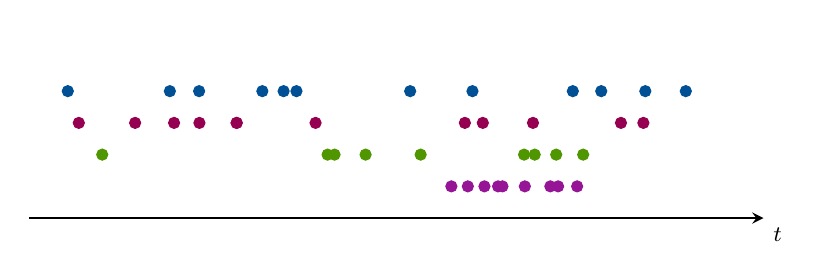
\begin{tikzpicture}
			  \begin{axis}[
		  width=0.9\columnwidth,
				  xlabel=$t$,
				  ymin = 0,
				  ymax = .6,
				  xmin = 0,
				  xmax=22,
				  xlabel style = {at={(axis cs:22,0)},anchor=north west},
				  y axis line style={draw=none},
				  x axis line style={->, thick},
				  ticks=none,
				  axis x line*=middle,
				  height=4cm,
				  ]
			  \addplot+[azulcito, mark options={fill=azulcito},mark=*,only marks] coordinates {
				  (1.168317969682793,0.4)
				  (4.224371806575089,0.4)
				  (5.099828260436964,0.4)
				  (6.9938720827411025,0.4)
				  (7.629926439960695,0.4)
				  (8.015139525296764,0.4)
				  (11.41978663218779,0.4)
				  (13.285132721106107,0.4)
				  (16.28953436494327,0.4)
				  (17.14081344555717,0.4)
				  (18.46073553951872,0.4)
				  (19.6728937320483,0.4)
			  };
			  \addplot+[rojito, mark options={fill=rojito},mark=*,only marks] coordinates {
				  (1.49783995292964,.3)
					(3.184138404294451,.3)
					(4.35051050123616,.3)
					(5.1091887517481505,.3)
					(6.221541171374557,.3)
					(6.226859317209702,.3)
					(8.586778366165495,.3)
				  (13.057655264423126,.3)
				   (13.594421727013588,.3)
				   (15.096680803679005,.3)
				  (17.731518813017008,.3)
				   (18.40246895328477,.3)				
			  };
		\addplot+[verdecito, mark options={fill=verdecito}, mark=*,only marks] coordinates {
				  (2.1995364349536235,0.2)
				  (8.947058606859512,0.2)
					(9.155089124125874,0.2)
				   (10.084686662202682,0.2)
				   (11.733424911823171,0.2)
				   (14.830631279727431,0.2)
				   (15.149252788554351,0.2)
				   (15.791821681936792,0.2)
				   (16.599742636184,0.2)
  
			  };
			  \addplot+[violetita,mark options={fill=violetita},mark=*,only marks] coordinates {
				  (12.653556737204989,0.1)
				   (13.146127585840045,0.1)
				   (13.643536674608884,0.1)
				   (14.051631664505377,0.1)
				   (14.183143031766923,0.1)
				   (14.85305783374829,0.1)
				   (15.61726438611725,0.1)
				   (15.848820745581179,0.1)
				   (16.419089799482926,0.1)
			  };
			  \end{axis}
		  \end{tikzpicture}
  
		
		\item At each point in time we must decide which items must be stored locally.

  	\end{myitem}
  
\end{frame}

  \begin{frame}{Two important distributions:}

	\begin{center}

		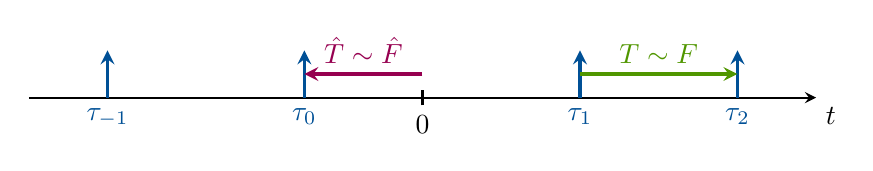
\begin{tikzpicture}
		   
			\draw[->,thick] (-5,0) -- (5,0);
			\node[below right] at (5,0) {$t$};
			
			\draw[<-,very thick, azulcito] (-4,.6) -- (-4,0) node[below] {$\tau_{-1}$};
			\draw[<-,very thick, azulcito] (-1.5,.6) -- (-1.5,0) node[below] {$\tau_{0}$};
			\draw[<-,very thick, azulcito] (2,.6) -- (2,0) node[below] {$\tau_{1}$};
			\draw[<-,very thick, azulcito] (4,.6) -- (4,0) node[below] {$\tau_{2}$};
			\draw[-,thick] (0,-.1) node[below] {$0$} -- (0,0.1);
			 
			\draw[->, very thick, verdecito] (2,.3) -- node[midway, above, anchor=south] {$T\sim F$} (4,.3);
	
			\draw<2->[->, very thick, rojito] (0,.3) -- node[midway, above, anchor=south] {$\hat{T}\sim \hat{F}$} (-1.5,.3);
	
		\end{tikzpicture}
	
	\end{center}

	\vfill

	\begin{itemize}
		\item \alert{Inter-arrival distribution:} Typical distance between points...
		 		\begin{equation*}
					X \sim F(t), \quad E[X] = 1/\lambda 
				\end{equation*} 
		\pause
		\item \alert{Age distribution:} Distance from the last point in the current interval (sampling bias)!
				\begin{equation*}
					\hat{X} \sim \hat{F}(t) := \lambda \int_0^t 1-F(s)ds,
				\end{equation*}
	\end{itemize}

		\vfill

		\pause
	{\footnotesize	\alert{Note:} you can formalize this under the \alert{Palm probability} framework for stationary point processes.}

\end{frame}

\section{Timer based caching}

\begin{frame}{Populating a cache: timer based (TTL) policies}
		
	\begin{itemize}
		\item<1-> Upon request arrival for item $i$, check for presence.
		\item<2-> If new, store item and start a \alert{timer} $T_i$ to evict.
		\item<3-> If present, reset timer to $T_i$.
		\item<4-> Upon timer expiration, evict the content.
		\item<5-> Keep timers $T_i$ such that \alert{average} cache occupation is $C$.
	\end{itemize}
	
	\vspace{3em}
	
	\centering
	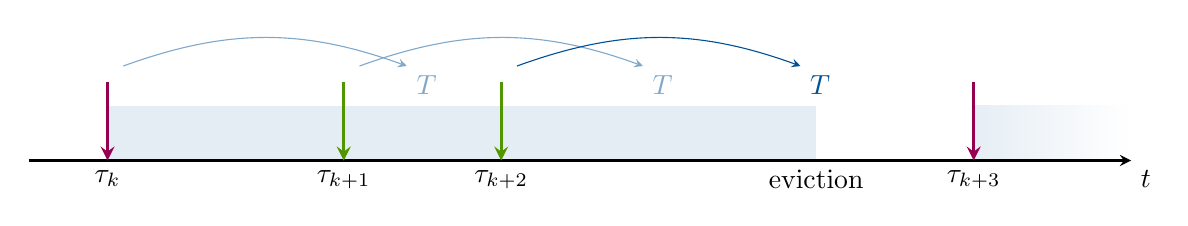
\begin{tikzpicture}
		\draw<4->[white,fill=azulcito!10!white] (1,.7) rectangle (10,0);
		\shade<5->[left color=azulcito!10!white, right color=white] (12,.7) rectangle (14,0);
	   
		\draw[->,thick] (0,0) -- (14,0);
		 \node[below right] at (14,0) {$t$};
		 
	   %  \draw[thick] (3,.1) -- (3,-.1);
	   %  \node[below left] at (3,0) {{\footnotesize $0$}};
	   
		 \draw<1->[->,very thick, rojito] (1,1) -- (1,0);
		 \draw<2-> [->,azulcito!50!white] (1.2,1.2) to [out=20,in=160] (4.8,1.2) node [below right] {$T$};
		 \draw<3->[->,very thick, verdecito] (4,1) -- (4,0);
		 \draw<3-> [->,azulcito!50!white] (4.2,1.2) to [out=20,in=160] (7.8,1.2) node [below right] {$T$};
		 \draw<3->[->,very thick, verdecito] (6,1) -- (6,0);
		 \draw<4-> [->,azulcito] (6.2,1.2) to [out=20,in=160] (9.8,1.2) node [below right] {$T$};
		 \draw<5->[->,very thick, rojito] (12,1) -- (12,0);
	   
		 \node<1->[below] at (1,0) {$\tau_k$};
		 \node<3->[below] at (4,0) {$\tau_{k+1}$};
		 \node<3->[below] at (6,0) {$\tau_{k+2}$};
		 \node<5->[below] at (12,0) {$\tau_{k+3}$};
		 \node<4->[below] at (10,0) {\alert{eviction}};
		 
		 
\end{tikzpicture}

\end{frame}

\begin{frame}{Hit and occupation probabilities}

	Focus on a single item $i$:

	\bigskip

	\begin{itemize}

		\item \alert{Hit probability:} prob. that \alert{next request} is still stored before timer expires:
			\begin{equation*}
				P(X_i<T_i) = F_i(T)
			\end{equation*}
		
		\item \alert{Memory usage:} prob. that item is stored at a random point in time, i.e. prob. that timer \alert{has not expired} since the last request:
		\begin{equation*}
			P(\hat{X}_i<T_i) = \hat{F}_i(T)
		\end{equation*}
	 
	\end{itemize}

\end{frame}


\begin{frame}{Choosing the optimal timers}

	Requests come from independent sources with intensities $\lambda_i$ and inter-arrival distribution $F_i$:

	\vfill

	\begin{problem}[Optimal TTL policy]
		Choose timers $T_i\geqslant 0$ such that:
		\begin{equation*}
			\max_{T_i\geqslant 0} \sum_i \lambda_i F_i (T_i)
		\end{equation*}
		subject to:
		\begin{equation*}
			\sum_i \hat{F}_i(T_i) \leqslant C
		\end{equation*}
	\end{problem}

	\vfill
	\alert{Remark:} non-convex non-linear program. But it can be solved by a change of variables!!! [Ferragut et al. -- QUESTA -- 2018].
\end{frame}

\begin{frame}{Structure of the optimal caching policy}

	\begin{itemize}
 	\item The crucial magnitude is the \alert{hazard rate} of $F$:
	\begin{equation*}
		\eta(t) := \frac{f(t)}{1-F(t)}
	\end{equation*}
	\item Likelihood of a request at time $t$, given the current interval has age $t$.
	\end{itemize}
	\pause

	\vfill

	\begin{theorem}[F', Rodriguez, Paganini -- 2016]

		If the $F_i$ have \alert{decreasing hazard rates}, then the optimal TTL policy satisfies:
			\begin{equation*}
				\eta_i (T_i^*) \geqslant \theta^*,
			   \end{equation*}
		whenever $T_i^*>0$ (i.e. the item is cached).
		
		Moreover, inequality is strict iff $T_i^*=\infty$ (item always stored).	  
	\end{theorem}

\end{frame}

\begin{frame}{Why caching helps in this case?}
	
	Decreasing hazard rates corresponds to \alert{bursty traffic}:

	\bigskip

	\begin{center}
		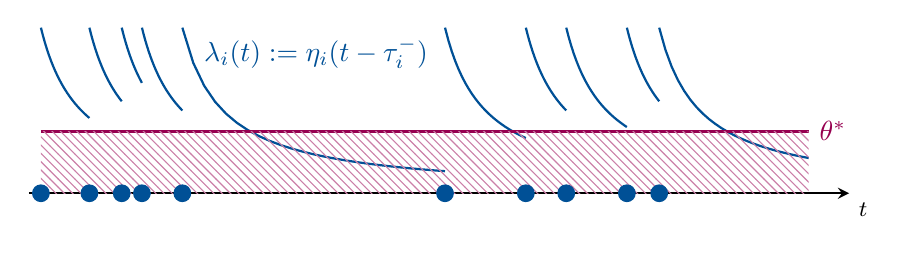
\begin{tikzpicture}
			\begin{axis}[xlabel=$t$,
				ymin = -.3,
				ymax = 2,
				xmin = -.3,
				xmax=20,
				xlabel style = {at={(axis cs:20,0)},anchor=north west},
				y axis line style={draw=none},
				x axis line style={->, thick},
				ticks=none,
				axis x line*=middle,
				width=12cm,
				height=4cm,
				]
				\addplot[azulcito,thick, domain=0:1.2] {2/(1+x)};
				\addplot[azulcito,thick, domain=1.2:2] {2/(1+x-1.2)};
				\addplot[azulcito,thick, domain=2:2.5] {2/(1+x-2)};
				\addplot[azulcito,thick, domain=2.5:3.5] {2/(1+x-2.5)};
				\addplot[azulcito,thick, domain=3.5:10] {2/(1+x-3.5)};
				\addplot[azulcito,thick, domain=10:12] {2/(1+x-10)};
				\addplot[azulcito,thick, domain=12:13] {2/(1+x-12)};
				\addplot[azulcito,thick, domain=13:14.5] {2/(1+x-13)};
				\addplot[azulcito,thick, domain=14.5:15.3] {2/(1+x-14.5)};
				\addplot[azulcito,thick, domain=15.3:19] {2/(1+x-15.3)};
				\node[below right, azulcito] at (axis cs:3.8,2) {$\lambda_i(t):=\eta_i(t-\tau_i^-)$};
				
				\addplot+[azulcito, mark options={fill=azulcito, scale=1.5}, mark=*,only marks] coordinates {
					(0,0)
					(1.2,0)
					 (2,0)
					 (2.5,0)
					 (3.5,0)
					 (10,0)
					 (12,0)
					 (13,0)
					 (14.5,0)
					 (15.3,0)
				};

				\draw<2->[rojito, very thick] (axis cs:0,.75) -- (axis cs:19,.75) node[right]{$\theta^*$};
				\path<3->[pattern=north west lines, pattern color=rojito!50!white] (axis cs:0,0.75) rectangle (19,0);
			\end{axis}
		\end{tikzpicture}
	\end{center}
	\pause
	\vfill

	\begin{itemize}
		\item<1-> An arrival makes a subsequent arrival \alert{more likely}.
		\item<2-> Store it while its likelihood is high enough (above a threshold).
	\end{itemize}
\end{frame}

\section{Timer based pre-fetching}

\begin{frame}{What about other types of traffic?}

	\begin{tabular}{m{7cm} m{6cm}}

		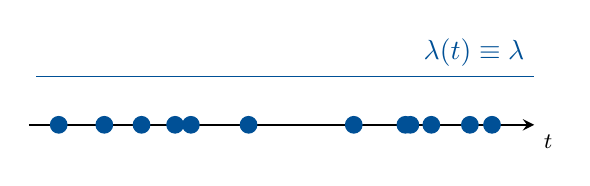
\begin{tikzpicture}
			\begin{axis}[xlabel=$t$,
				ymin = -.3,
				ymax = 2,
				xmin = -.3,
				xmax=20,
				xlabel style = {at={(axis cs:20,0)},anchor=north west},
				y axis line style={draw=none},
				x axis line style={->, thick},
				ticks=none,
				axis x line*=middle,
				width=8cm,
				height= 3cm,
				]
				\addplot[azulcito, domain=0:20] {1};
				\node[above left, azulcito] at (axis cs:20,1) {$\lambda(t)\equiv \lambda$};
	
				\addplot+[azulcito, mark options={fill=azulcito, scale=1.5}, mark=*,only marks] coordinates {
					(0.9028581008067987,0)
					(2.7341797790213573,0)
					(4.228330726726128,0)
					(5.577074925845067,0)
					(6.211423990911654,0)
					(8.528255357570485,0)
					(12.753859672976413,0)
					(14.826517141978712,0)
					(15.028110470502309,0)
					(15.868264106338712,0)
					(17.418133532477547,0)
					(18.306210880027027,0)
				};
			\end{axis}
		\end{tikzpicture} & \alert{Constant hazard rate} $\to$ Poisson process.\\
		\\
		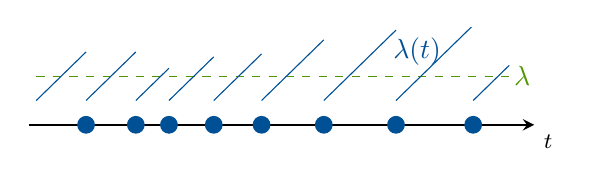
\begin{tikzpicture}
			\begin{axis}[xlabel=$t$,
				ymin = -.3,
				ymax = 2,
				xmin = -.3,
				xmax=20,
				xlabel style = {at={(axis cs:20,0)},anchor=north west},
				y axis line style={draw=none},
				x axis line style={->, thick},
				ticks=none,
				axis x line*=middle,
				width=8cm,
				height=3cm,
				]
				\addplot[verdecito,domain=0:19, dashed] {1};
				\addplot[azulcito,domain=0:2] {0.5+0.5*x};
				\addplot[azulcito,domain=2:4] {0.5+0.5*(x-2};
				\addplot[azulcito,domain=4:5.33] {0.5+0.5*(x-4};
				\addplot[azulcito,domain=5.33:7.13] {0.5+0.5*(x-5.33};
				\addplot[azulcito,domain=7.13:9.05] {0.5+0.5*(x-7.13};
				\addplot[azulcito,domain=9.05:11.55] {0.5+0.5*(x-9.05};
				\addplot[azulcito,domain=11.55:14.45] {0.5+0.5*(x-11.55};
				\addplot[azulcito,domain=14.45:17.55] {0.5+0.5*(x-14.45};
				\addplot[azulcito,domain=17.55:19] {0.5+0.5*(x-17.55};
				\node[below, azulcito] at (axis cs:15.3,2) {$\lambda(t)$};
				\node[right, verdecito] at (axis cs:18.8,1) {$\lambda$};

				\addplot+[azulcito, mark options={fill=azulcito, scale=1.5}, mark=*,only marks] coordinates {
					(2,0)
					(4,0)
					(5.33,0)
					(7.13,0)
					(9.05,0)
					(11.55,0)
					(14.45,0)
					(17.55,0)
				};
			\end{axis}
		\end{tikzpicture} & \alert{Increasing} hazard rate $\to$ more periodic!\\

	\end{tabular}

	\vfill

	\pause

	\alert{Theorem:} for these types of traffic, keep the most popular is the optimal \alert{caching} policy.

	\vfill

	\pause

	\begin{center}
		\alert{Can we improve upon this?}
	\end{center}

\end{frame}


\begin{frame}{Thinking about increasing hazard rates...}

	\begin{itemize}
	\item Once you have seen a request, it's \alert{less likely} to see the same item again for a while.
	
		\bigskip

	\begin{center}
	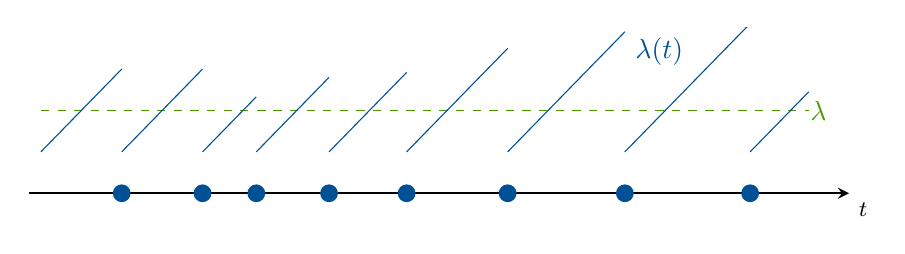
\begin{tikzpicture}
		\begin{axis}[xlabel=$t$,
			ymin = -.3,
			ymax = 2,
			xmin = -.3,
			xmax=20,
			xlabel style = {at={(axis cs:20,0)},anchor=north west},
			y axis line style={draw=none},
			x axis line style={->, thick},
			ticks=none,
			axis x line*=middle,
			width=12cm,
			height=4cm,
			]
			\addplot[verdecito,domain=0:19, dashed] {1};
			\addplot[azulcito,domain=0:2] {0.5+0.5*x};
			\addplot[azulcito,domain=2:4] {0.5+0.5*(x-2};
			\addplot[azulcito,domain=4:5.33] {0.5+0.5*(x-4};
			\addplot[azulcito,domain=5.33:7.13] {0.5+0.5*(x-5.33};
			\addplot[azulcito,domain=7.13:9.05] {0.5+0.5*(x-7.13};
			\addplot[azulcito,domain=9.05:11.55] {0.5+0.5*(x-9.05};
			\addplot[azulcito,domain=11.55:14.45] {0.5+0.5*(x-11.55};
			\addplot[azulcito,domain=14.45:17.55] {0.5+0.5*(x-14.45};
			\addplot[azulcito,domain=17.55:19] {0.5+0.5*(x-17.55};
			\node[below, azulcito] at (axis cs:15.3,2) {$\lambda(t)$};
			\node[right, verdecito] at (axis cs:18.8,1) {$\lambda$};

			\addplot+[azulcito, mark options={fill=azulcito, scale=1.5}, mark=*,only marks] coordinates {
				(2,0)
				(4,0)
				(5.33,0)
				(7.13,0)
				(9.05,0)
				(11.55,0)
				(14.45,0)
				(17.55,0)
			};
		\end{axis}
	\end{tikzpicture}
	\end{center}

	
	
	\item What is the timer based equivalent of this case?
	\end{itemize}

	\pause
	\vfill

	\begin{block}{Key insight}
		The question now is not \alert{how long we should remember something}, but instead \alert{how long we should forget about it}!
	\end{block}
		
\end{frame}

\begin{frame}{Timer based pre-fetching policy}


\begin{itemize}
	\item<1-> Upon request arrival for item $i$, check for presence.
	\item<2-> If not-present:  start a \alert{timer} $T_i$.
	\item<3-> If present: remove content and reset timer to $T_i$.
	\item<4-> Upon timer expiration, \alert{pre-fetch} the content.
	\item<5-> Keep timers $T_i$ such that \alert{average} cache occupation is $C$.
\end{itemize}

\vspace{3em}

\centering

\input{figuras/ttl_pre.tikz}

\end{frame}

\begin{frame}{Timer based pre-fetching}
	
	Consider a single item with a timer $T$ and its request process:

	\bigskip

	\begin{columns}[T]
		\begin{column}{.5\textwidth}
		\textbf{Hit probability:} \alert{next} arrival occurs \alert{after} timer expires.

		\bigskip
		
		\begin{center}

		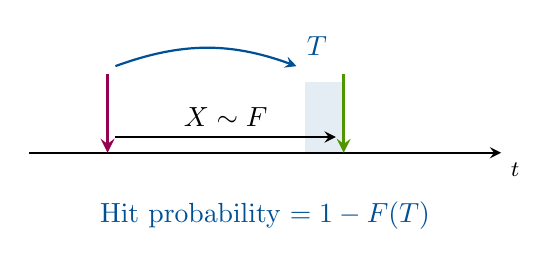
\begin{tikzpicture}[scale=1]
			\draw[white,fill=azulcito!10!white] (3.5,.9) rectangle (4,0);
		  \draw[->,thick] (0,0) -- (6,0);
		  \node[below right] at (6,0) {\footnotesize $t$};
		
		  \draw[->,very thick, rojito] (1,1) -- (1,0);
		  \draw [->,thick,azulcito] (1.1,1.1) to [out=20,in=160] (3.4,1.1) node [above right] {$T$};
		  \draw [->,thick,black] (1.1,.2) -- (3.9,.2) node [above, midway] {$X \sim F$};
		  \draw[->,very thick, verdecito] (4,1) -- (4,0);
		  \node[azulcito,below] at (3,-.5) {Hit probability $=1-F(T)$};
		  \end{tikzpicture}
		  \end{center}
		
		\end{column}
		
		\begin{column}{0.5\textwidth}

		\textbf{Occupation probability:} probability that timer \alert{has} expired by $0$ since last arrival.

		\begin{center}

		 \bigskip

		 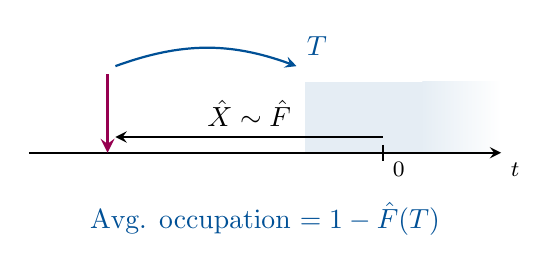
\begin{tikzpicture}
		 \draw[white,fill=azulcito!10!white] (3.5,0.9) rectangle (5,0); 
		 \shade[left color=azulcito!10!white, right color=white] (5,.9) rectangle (6,0);
		  \draw[->,thick] (0,0) -- (6,0);
		  \node[below right] at (6,0) {\footnotesize $t$};
		  
		  \draw[thick] (4.5,.1) -- (4.5,-.1);
		  \node[below right] at (4.5,0) {{\footnotesize $0$}};
		
		  \draw[->,very thick, rojito] (1,1) -- (1,0);
		  \draw [->,thick,azulcito] (1.1,1.1) to [out=20,in=160] (3.4,1.1) node [above right] {$T$};		 % \draw[->,very thick, rojito!20!white] (5.75,1) -- (5.75,0);
		  \draw [<-,thick, black] (1.1,.2) -- (4.5,.2) node [above, midway] {$\hat{X}\sim\hat{F}$};
		  
		  \node[azulcito,below] at (3,-.5) {Avg. occupation $= 1-\hat{F}(T)$};
		\end{tikzpicture}
		\end{center}
		
		\end{column}
		\end{columns}
\end{frame}

\begin{frame}{Choosing the optimal timers}

	Requests come from independent sources with intensities $\lambda_i$ and inter-arrival distribution $F_i$:

	\vfill

	\only<1>{
	\begin{problem}[Optimal pre-fetching policy]
		Choose timers $T_i\geqslant 0$ such that:
		\begin{equation*}
			\max_{T_i\geqslant 0} \sum_i \lambda_i (1-F_i(T_i))
		\end{equation*}
		subject to:
		\begin{equation*}
			\sum_i (1-\hat{F}_i(T_i)) \leqslant C
		\end{equation*}
	\end{problem}
	}
	\only<2->{
		\begin{problem}[Optimal pre-fetching policy]
			Choose timers $T_i\geqslant 0$ such that:
			\begin{equation*}
				\min_{T_i\geqslant 0} \sum_i \lambda_i F_i(T_i)
			\end{equation*}
			subject to:
			\begin{equation*}
				\sum_i \hat{F}(T_i) \geqslant N-C
			\end{equation*}
		\end{problem}		
	}
	\vfill
	\pause
	\alert{Remark:} we can use the same change of variables again!
\end{frame}

\begin{frame}{Choosing the optimal timers}{Change of variables}
	
	\begin{myitem}[2em]
	\item Apply the change of variables $u_i = \hat{F}_i(T_i)$. 
	\item Note that $u_i$ is the probability of \alert{not being stored}. 
	
	\item The problem becomes:
	\begin{equation*}
		\min_{u_i \in [0,1]} \sum_i \lambda_i F_i(\hat{F}^{-1}_i(u_i))
	\end{equation*}
	subject to:
	\begin{equation*}
		\sum_i u_i \geqslant N-C
	\end{equation*}

	\end{myitem}

\end{frame}

\begin{frame}{Choosing the optimal timers}{Lagrangian duality}

	\begin{itemize}
		\item Objective gradient:
		\begin{equation*}
			\frac{\partial}{\partial u_i} \lambda_i F_i\circ\hat{F}^{-1}_i(u_i) = \frac{\lambda_i f_i(\hat{F}^{-1}_i(u_i))}{\lambda_i \left(1-F_i(\hat{F}^{-1}_i(u_i))\right)} = \eta_i(\hat{F}^{-1}_i(u_i))
		\end{equation*}

		\item \alert{Increasing!} $\to$ Proper convex optimization problem.
		
		\pause

		\item Lagrangian duality:
		
		\begin{align*}
  			\mathcal{L}(u,\theta) =& \sum_{i=1}^N \lambda_i F_i\left(\hat{F}^{-1}_i(u_i)\right) + \theta \left(N-C - \sum_{i=1}^N u_i\right) \\
			=& \sum_{i=1}^N \left[\lambda_i F_i\left(\hat{F}^{-1}_i(u_i)\right) - \theta u_i \right] + \theta (N-C).
		\end{align*}

	\end{itemize}

\end{frame}

\begin{frame}{Main result}

	\begin{theorem}
		If the $F_i$ satisfy the IHR property, there exists a unique threshold $\theta^*\geqslant 0$ such that the optimal timers satisfy:
		\begin{equation*}
		  \eta_i(T_i^*) \geqslant \theta^*,
		\end{equation*}
		whenever $T_i^*<\infty$ (pre-fetching). 
		
		The inequality is strict if and only if $T_i^*=0$, i.e. the content is always stored.
	\end{theorem}

	\pause

	\vfill
	
	
	\alert{Remark:} Again the policy is a threshold policy.

\end{frame}


\begin{frame}{Simulation example}
	
	Erlang ($k=5$) inter-arrival times, Zipf $\propto n^{-\beta}$ popularities, varying $\beta$, $N=10000$, $C=1000$.

\begin{center}
\includegraphics[width=0.7\textwidth]{figuras/comparison.pdf}
\end{center}

\vfill
\begin{itemize}
\item Pre-fetching improves over the static policy.
\item Classical caching (e.g. LRU) is a very bad idea for regular traffic.
\end{itemize}
\end{frame}

\begin{frame}{A tale of two policies...}


	\begin{columns}
		\begin{column}{0.65\textwidth}
			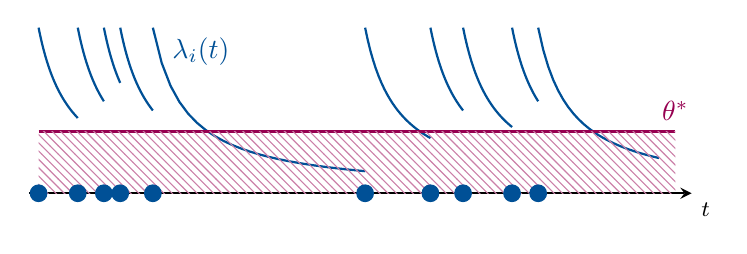
\begin{tikzpicture}
				\begin{axis}[xlabel=$t$,
					ymin = -.3,
					ymax = 2,
					xmin = -.3,
					xmax=20,
					xlabel style = {at={(axis cs:20,0)},anchor=north west},
					y axis line style={draw=none},
					x axis line style={->, thick},
					ticks=none,
					axis x line*=middle,
					width=10cm,
					height=4cm,
					]
					\addplot[azulcito,thick, domain=0:1.2] {2/(1+x)};
					\addplot[azulcito,thick, domain=1.2:2] {2/(1+x-1.2)};
					\addplot[azulcito,thick, domain=2:2.5] {2/(1+x-2)};
					\addplot[azulcito,thick, domain=2.5:3.5] {2/(1+x-2.5)};
					\addplot[azulcito,thick, domain=3.5:10] {2/(1+x-3.5)};
					\addplot[azulcito,thick, domain=10:12] {2/(1+x-10)};
					\addplot[azulcito,thick, domain=12:13] {2/(1+x-12)};
					\addplot[azulcito,thick, domain=13:14.5] {2/(1+x-13)};
					\addplot[azulcito,thick, domain=14.5:15.3] {2/(1+x-14.5)};
					\addplot[azulcito,thick, domain=15.3:19] {2/(1+x-15.3)};
					\node[below right, azulcito] at (axis cs:3.8,2) {$\lambda_i(t)$};
					
					\addplot+[azulcito, mark options={fill=azulcito, scale=1.5}, mark=*,only marks] coordinates {
						(0,0)
						(1.2,0)
						 (2,0)
						 (2.5,0)
						 (3.5,0)
						 (10,0)
						 (12,0)
						 (13,0)
						 (14.5,0)
						 (15.3,0)
					};
	
					\draw<2->[rojito, very thick] (axis cs:0,.75) -- (axis cs:19.5,.75) node[above]{$\theta^*$};
					\path<2->[pattern=north west lines, pattern color=rojito!50!white] (axis cs:0,0.75) rectangle (19.5,0);
				\end{axis}
			\end{tikzpicture}

			\vspace{2em}

			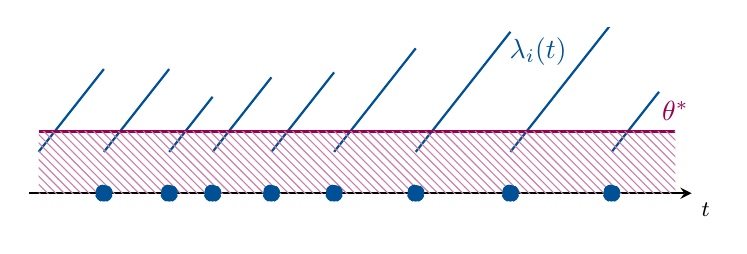
\begin{tikzpicture}
				\begin{axis}[xlabel=$t$,
					ymin = -.3,
					ymax = 2,
					xmin = -.3,
					xmax=20,
					xlabel style = {at={(axis cs:20,0)},anchor=north west},
					y axis line style={draw=none},
					x axis line style={->, thick},
					ticks=none,
					axis x line*=middle,
					width=10cm,
					height=4cm,
					]
					\addplot[azulcito, thick, domain=0:2] {0.5+0.5*x};
					\addplot[azulcito,thick, domain=2:4] {0.5+0.5*(x-2};
					\addplot[azulcito,thick, domain=4:5.33] {0.5+0.5*(x-4};
					\addplot[azulcito,thick, domain=5.33:7.13] {0.5+0.5*(x-5.33};
					\addplot[azulcito,thick, domain=7.13:9.05] {0.5+0.5*(x-7.13};
					\addplot[azulcito,thick, domain=9.05:11.55] {0.5+0.5*(x-9.05};
					\addplot[azulcito,thick, domain=11.55:14.45] {0.5+0.5*(x-11.55};
					\addplot[azulcito,thick, domain=14.45:17.55] {0.5+0.5*(x-14.45};
					\addplot[azulcito,thick, domain=17.55:19] {0.5+0.5*(x-17.55};
					\node[below, azulcito] at (axis cs:15.3,2) {$\lambda_i(t)$};

					\addplot+[azulcito, mark options={fill=azulcito, scale=1.5}, mark=*,only marks] coordinates {
				(2,0)
				(4,0)
				(5.33,0)
				(7.13,0)
				(9.05,0)
				(11.55,0)
				(14.45,0)
				(17.55,0)
			};
			
					\draw<2->[rojito, very thick] (axis cs:0,.75) -- (axis cs:19.5,.75) node[above]{$\theta^*$};
					\path<2->[pattern=north west lines, pattern color=rojito!50!white] (axis cs:0,0.75) rectangle (19.5,0);
				\end{axis}
			\end{tikzpicture}
		\end{column}
		\begin{column}{0.35\textwidth}

			 \uncover<2->{
				Both policies are just the same policy!

				\bigskip

				\begin{itemize}
					\item Keep a hazard rate threshold $\theta$ for storing a content
					
					\item Compute $\theta^*$ such that avg. memory occupation is $C$.
				\end{itemize}
			 }
		\end{column}
	\end{columns}

\end{frame}

\section{Asymptotic optimality}

\begin{frame}{Asymptotic optimality}

	\begin{itemize}

		\item Threshold policies in fact are related to recent results by [Panigrahy et al. 2022], about the optimal causal policy.
		
		\item They also identify a notion of \emph{hazard rate}, the stochastic intensity, as defininf the optimal policy.

	\end{itemize}

	\pause
	\vfill

	\begin{theorem}[F', Carrasco, Paganini -- In preparation -- check ArXiv soon]

		Under an appropriate scaling regime, as $N\to\infty$ and $C=cN$, the optimal causal policy converges to a \alert{fixed threshold policy}. Moreover, the limit threshold $\theta^*$ coincides with its timer based counterpart.
	\end{theorem}
	
	\vfill
	
	Therefore, the above policies give a \alert{universal asymptotic upper bound} on caching performance.
\end{frame}

\section{Final remarks}

\begin{frame}{Final remarks}
	
	\begin{myitem}[2em]
		\item<1-> You have to \alert{know your traffic} before deciding on caching or pre-fetching!
		
		\item<2-> Classical caching is \alert{not well suited} to regular traffic.
		
		\item<3-> We identified the \alert{hazard rate} as the crucial indicator of regularity, and devised a new policy for IHR, that is also \alert{asymptotically optimal} among all causal policies.
		
		\item<4-> A lot of open questions, in particular:
		
		\pause

		\begin{itemize}
			\item How we can learn the hazard rates online?
			\item How we can estimate the appropriate threshold?
			\item What about mixtures of IHR and DHR traffic?
		\end{itemize}

		\pause


	\end{myitem}
\end{frame}


\begin{frame}[plain]
	\vfill
	{\Huge \alert{Tante grazie!}}
	\vfill
	Andres Ferragut (and Diego Goldsztajn)

	\smallskip

	\href{mailto://ferragut@ort.edu.uy}{\alert{ferragut@ort.edu.uy}}
	
	\smallskip

	\href{http://aferragu.github.io}{\alert{aferragu.github.io}}
\end{frame}

\begin{frame}[allowframebreaks]{References}

	\begin{thebibliography}{1}

		\bibitem{bremaud2020point}
		P.~Brémaud.
		\newblock {\em Point process calculus in time and space}.
		\newblock Springer, NY, 2020.
		
		\bibitem{che2002hierarchical}
		H.~Che, Y.~Tung, and Z.~Wang.
		\newblock Hierarchical web caching systems: Modeling, design and experimental results.
		\newblock {\em IEEE Journal on Selected Areas in Communications}, 20(7):1305--1314, 2002.
		
		\bibitem{ferragut2016caches_sigmetrics}
		A.~Ferragut, I.~Rodriguez, and F.~Paganini.
		\newblock Optimizing {TTL} caches under heavy tailed demands.
		\newblock In {\em Proc. of ACM/SIGMETRICS 2016}, pages 101--112, June 2016.
		
		\bibitem{ferragut2018optimal}
		A.~Ferragut, I.~Rodríguez, and F.~Paganini.
		\newblock Optimal timer-based caching policies for general arrival processes.
		\newblock {\em Queueing Systems}, 88(3--4):207--241, 2018.
		
		\bibitem{fofack2014performance}
		N.~C. Fofack, P.~Nain, G.~Neglia, and D.~Towsley.
		\newblock Performance evaluation of hierarchical {TTL}-based cache networks.
		\newblock {\em Computer Networks}, 65:212--231, 2014.
		
		\bibitem{panigrahy2022upper}
		N.~K. Panigrahy, P.~Nain, G.~Neglia, and D.~Towsley.
		\newblock A new upper bound on cache hit probability for non-anticipative caching policies.
		\newblock {\em ACM Trans. Model. Perform. Eval. Comput. Syst.}, 7(2--4), November 2022.
		
		\end{thebibliography}
	
		\vfill

\end{frame}
\end{document}
